%!TEX TS-program = xelatex
\documentclass[]{friggeri-cv}

\usepackage{afterpage}
\usepackage{hyperref}
\usepackage{color}
\usepackage{xcolor}
\definecolor{myblue}{RGB}{4, 98, 249}
\usepackage{hyperref}
\hypersetup{
    pdftitle={},
    pdfauthor={},
    pdfsubject={},
    pdfkeywords={},
    colorlinks=true,       % no lik border color
    allbordercolors=white    % white border color for all
}
\addbibresource{bibliography.bib}
\RequirePackage{xcolor}
\definecolor{pblue}{HTML}{0395DE}


% ------------
\usepackage{enumitem}
\renewenvironment{entrylist}{%
  \begin{itemize}[leftmargin=1in]%[leftmargin=*,align=left,itemindent=-\dimexpr\labelwidth+\labelindent+\labelsep\relax]
  }{%
  \end{itemize}
}
\renewcommand{\bfseries}{\headingfont\color{headercolor}}
\renewcommand{\entry}[4]{%
\item[#1]
  \textbf{#2}%
  \hfill%
  {\footnotesize\addfontfeature{Color=myblue} #3}\\%
  #4\vspace{\parsep}%
}
% -------


\begin{document}
%\header{Boyang}{Yan}

\section{Personal Information}
\begin{tabular}{p{3cm} p{3cm} p{3cm} p{3cm} }
  \textbf{Name}: & Boyang Yan & \textbf{Gender}: & Male \\
  \textbf{DOB}:  & July 13, 1993  &  \textbf{Nationality}: & Chinese \\
  \textbf{Blog}:  & \href{http://www.yanboyang.com}{yanboyang.com} &  & \\
\end{tabular}

% Fake text to add separator      
\fcolorbox{white}{gray}{\parbox{\dimexpr\textwidth-2\fboxsep-2\fboxrule}{%
.....
}}

% In the aside, each new line forces a line break
\begin{aside}
  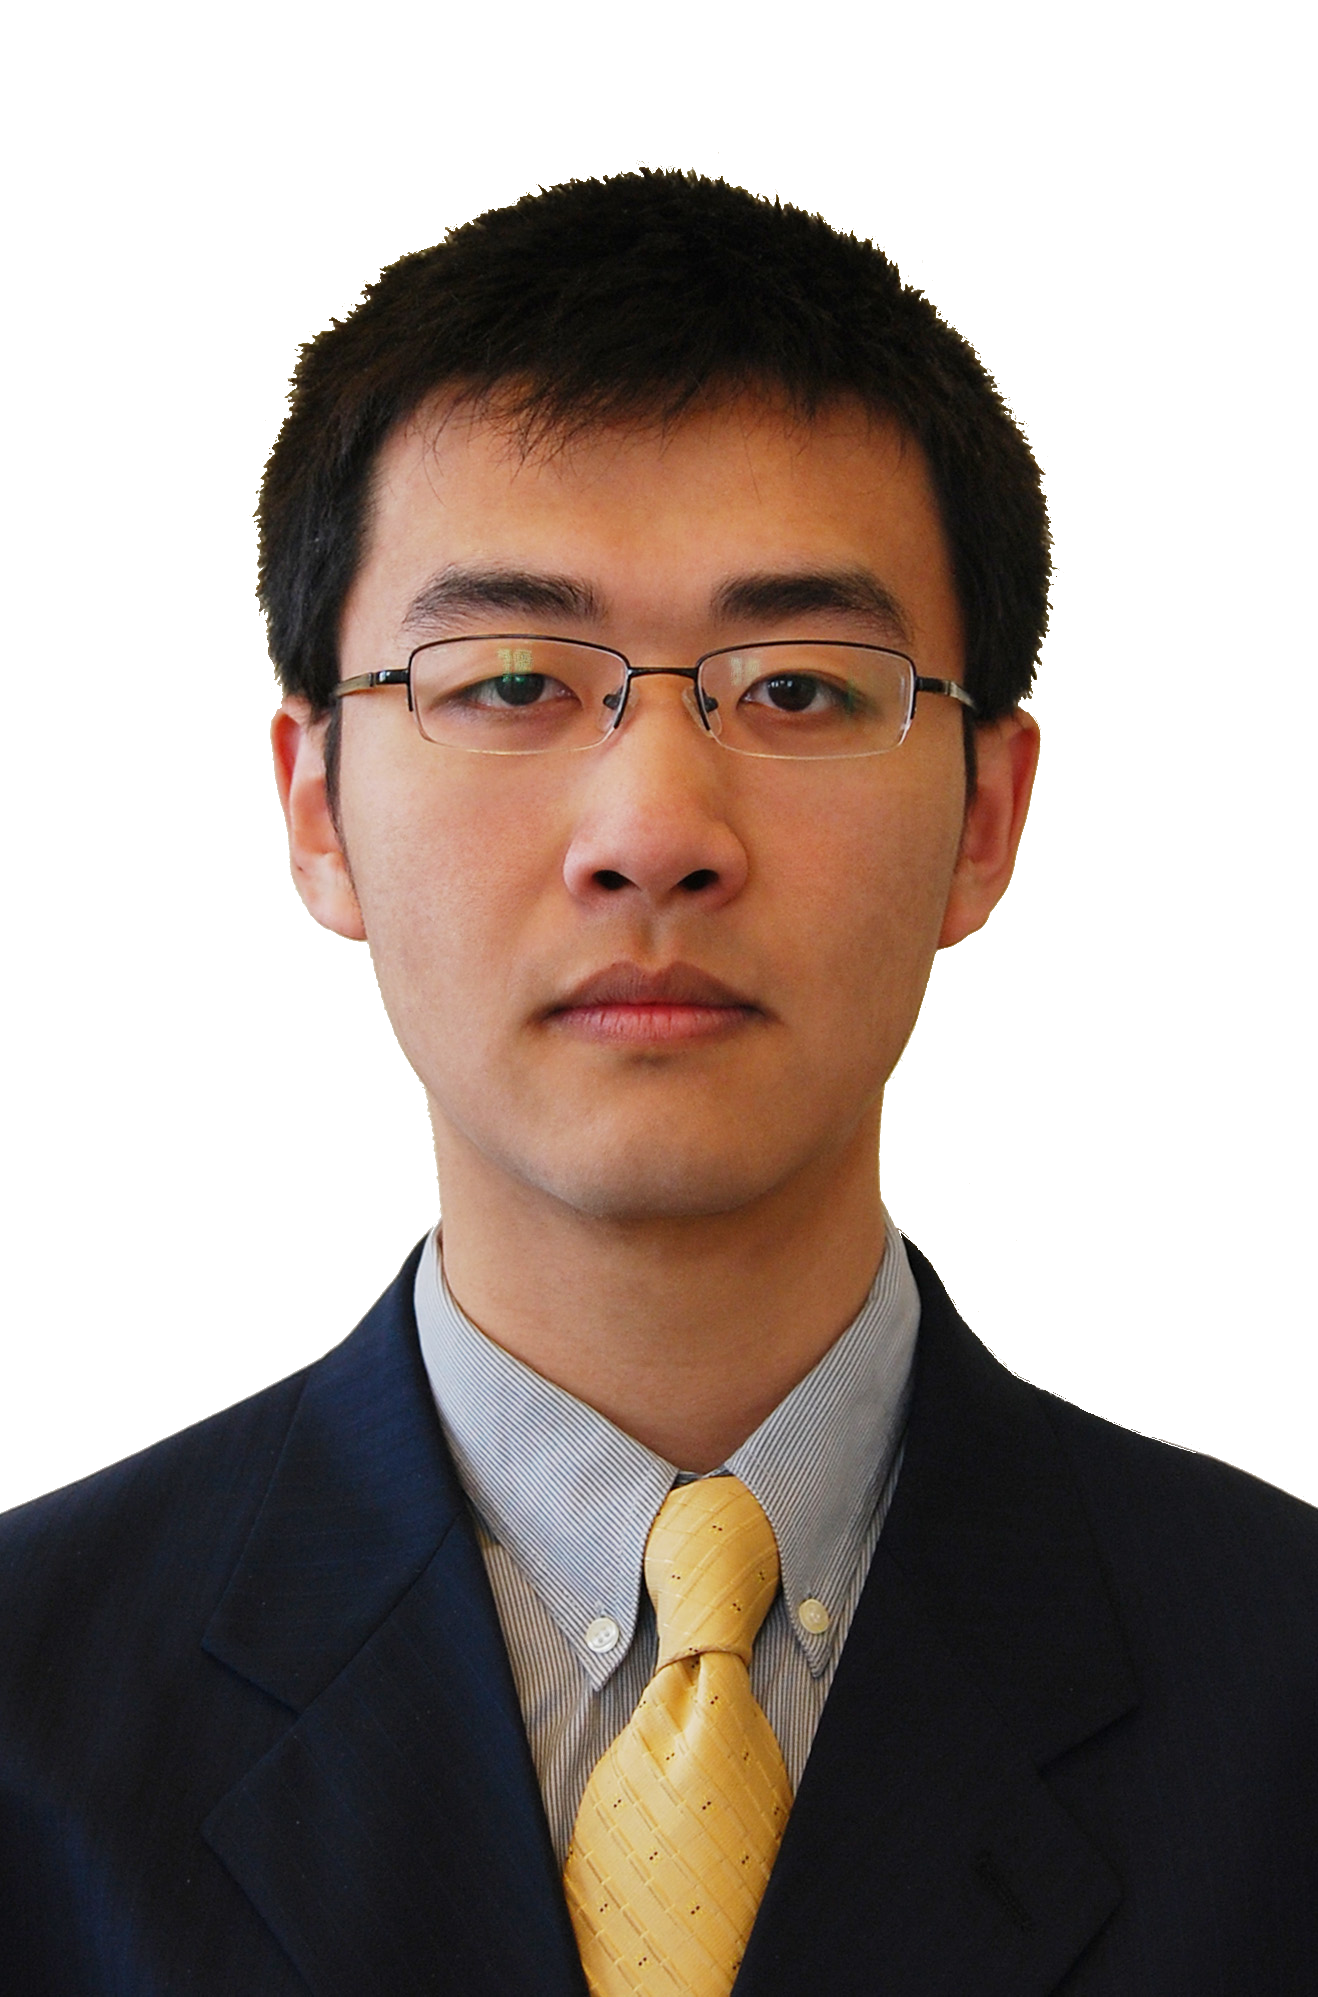
\includegraphics[scale=0.007]{img/boyang.png}
  \section{Address}
  14-6-602 Zhuhuali Community, Huayuanxincheng
  Nankai District,  Tianjin,
  China
    ~
  \section{Contact Info}
  \textbf{Tel:} +86 18512290791
    \textbf{Wechat:} yanboyang713
    ~
  \section{E-mail}
    \href{mailto:yanboyang713@gmail.com}{\textbf{yanboyang713@}\\gmail.com}
    ~
  \section{Blog \& GitHub}
    \href{https://github.com/yanboyang713}{github.com/yanboyang713}
    \href{http://www.yanboyang.com}{yanboyang.com}
    ~
  \section{Programming}
    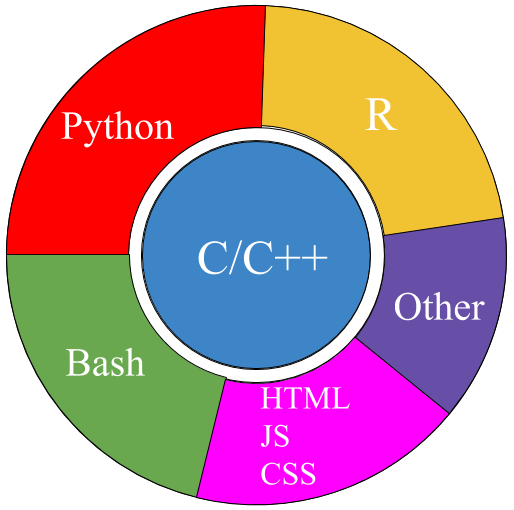
\includegraphics[scale=0.2]{img/programming.png}
    ~
  \section{OS Preference}
    \textbf{GNU/Linux}
\includegraphics[scale=0.40]{img/5stars.png}
    \textbf{Unix}
\includegraphics[scale=0.40]{img/4stars.png}
    \textbf{MacOS}
\includegraphics[scale=0.40]{img/3stars.png}
    \textbf{Windows}
\includegraphics[scale=0.40]{img/1stars.png}
    ~
    \section{Languages}
    \textbf{Chinese}
\includegraphics[scale=0.40]{img/5stars.png}
    \textbf{English}
\includegraphics[scale=0.40]{img/4stars.png}
    ~
\end{aside}

\section{Overview}
I see myself advancing with strong ability, and passion for new technology and
academic research. I have three years of working experience in Machine Learning
and Software Testing at Microsoft and research institution. Also, I like to
write my blog every week to share some of my new readings and findings.

\textbf{Areas of Interest}: Machine Learning, Computer Graphics, Simultaneous
localization and mapping (SLAM)

\section{Working Experience}
\begin{entrylist}
  \entry
  {\footnotesize{Mar, 2020 - Jun, 2021}\\}
  {\large{Support Engineer}}
  {Microsoft, China}
  {The architecture of Azure public cloud to support Machine Learning algorithm,
    based on different Azure Service such as Azure Data Lake, Azure Batch, Azure Kubernetes, Azure Edge and Azure Networking etc.\\}
\end{entrylist}

\begin{entrylist}
  \entry
  {\footnotesize{Dec, 2018 - Mar, 2020}\\}
  {\large{Algorithm Engineer}}
  {Peng Chen Laboratory, Shenzhen, China}
  { Flight Control System Testing for fixed-wing UAV (Ardupilot), 3D Printing\\}
\end{entrylist}

\begin{entrylist}
  \entry
  {\footnotesize{Jan, 2018 - Nov, 2018}\\}
  {\large{Research Assistant (Computer Science)}\\}
  {University of Wollongong, Australia}
  { Metamorphic Testing - Software Testing, Big Data Analysis, Natural Language Processing\\}
\end{entrylist}


\section{Education}
\begin{entrylist}
  \entry
  {\footnotesize{Mar, 2021 - now}\\}
    {\large{Master of Statistics and Operations Research}\\}
    {Royal Melbourne Institute of Technology (RMIT), Australia}

  \entry
  {\footnotesize{Mar, 2014 - Dec, 2017}\\}
    {\large{Bachelor of Computer Science}\\​}
    {University of Wollongong, Australia}
    {Major in Software Engineering}
    
  \entry
  {\footnotesize{Mar, 2013 - Mar, 2014}\\}
  {\large{English for Tertiary Studies (Academic English)}\\}
  {University of Wollongong College, Australia}

  \entry
  {\footnotesize{Sep, 2011 - Mar, 2013}\\}
    {\large{Bachelor of Business Management}\\}
    {China University Of Mining And Technology}

  \end{entrylist}
  
\section{Publications}
2019 \textbf{\textcolor{black}{Boyang Yan}}, Brian Yecies, Zhi Quan Zhou*: Metamorphic Relations for Data
Validation: A Case Study of Translated Text Messages. IEEE/ACM 4th International
Workshop on Metamorphic Testing (MET '19), in conjunction with the 41st
International Conference on Software Engineering (ICSE '19).

%\newpage

\section{Patents}
\begin{entrylist}

  \entry
  {June 2, 2020\\}
  {An automated text difference analysis and verification system/method\\}
  {Principal inventor of the patent}
  {China Patent Office Application ID: 202010489931.8}

\end{entrylist}

\section{Academy Congress and Conference}
\begin{entrylist}
  \entry
  {May 26, 2019}
  {Boyang Yan, Brian Yecies, Zhi Quan Zhou* -
    Title: Metamorphic Relations for Data Validation: A Case Study of Translated
    Text Messages. (Paper Presentation and Speech)}
  {ICSE, Montreal, Canada}

  \entry
  {August 11, 2017}
  {Boyang Yan - Title: Human Resource Management
      System based on Web. (Poster)}
  {IEEE Sections Congress (SC2017), Sydney, Australia}

\end{entrylist}

\section{Awards and Achievements}\begin{entrylist}
  \entry
  {2020}
  {Microsoft Hackathon Prize}
  {Microsoft, China}

  \entry
  {2019}
  {First Aid CPR AED\\}
  {American Heart Association}
  
  \entry
  {2018}
  {The best undergraduate final project prize}
  {University of Wollongong, Australia}
  
  \entry
  {2018}
  {Publicly acknowledged in the “Acknowledgements” section of following research paper:}
    {ICSE}
    {2018 D. Pesu, Z. Q. Zhou*, J. Zhen, and D. Towey: A Monte Carlo method for metamorphic testing of machine
      translation services,” in Proceedings of the IEEE/ACM 3rd International Workshop on Metamorphic Testing
      (MET ’18), in conjunction with the 40th International Conference on Software Engineering (ICSE ’18).}
  
  \entry
  {2017}
  {Amateur Radio Operator's certificate of proficiency (Standard)\\}
  {The Wireless Institute of Australia (WIA)}

  \entry
  {2014, 2015}
  {Undergraduate Excellence Scholarship}
  {University of Wollongong, Australia}
 
\end{entrylist}

%%% This piece of code has been commented by Karol Kozioł due to biblatex errors. 
% 
%\printbibsection{article}{article in peer-reviewed journal}
%\begin{refsection}
%  \nocite{*}
%  \printbibliography[sorting=chronological, type=inproceedings, title={international peer-reviewed conferences/proceedings}, notkeyword={france}, heading=subbibliography]
%\end{refsection}
%\begin{refsection}
%  \nocite{*}
%  \printbibliography[sorting=chronological, type=inproceedings, title={local peer-reviewed conferences/proceedings}, keyword={france}, heading=subbibliography]
%\end{refsection}
%\printbibsection{misc}{other publications}
%\printbibsection{report}{research reports}

\end{document}
